% FYP mid-semester progress presentation (integration \& full testing still in progress)

\documentclass[aspectratio=169]{beamer}
\usetheme{Madrid}
\usecolortheme{default}
\setbeamertemplate{navigation symbols}{}
\setbeamertemplate{footline}{}

\title{Deploying an Autonomous Indoor Robot with Laser Mapping and Multi-Hop Networking for Disaster Site Exploration}
\subtitle{Progress Presentation}
\author{
  Habeel Ali (FA22-BCE-067) \\
  Tahreem Shahid (FA22-BCE-035) \\
  Ramisha Ikram (FA22-BCE-024) \\
  Ibrahim Imran (FA22-BCE-032)
}
\date{}
\institute{FYP Progress}

\usepackage{graphicx}
\usepackage{booktabs}

\begin{document}

\begin{frame}
\titlepage
\end{frame}

\begin{frame}{Outline}
\begin{itemize}
\item Current status (completed vs.\ pending)
\item Literature review
\item Problem \& objectives
\item Methodology (SLAM, communication, perception)
\item Implementation (platform \& stack)
\item Results (mapping, communication, perception)
\item Remaining work \& conclusions
\end{itemize}
\end{frame}

% --- Current status ---
\begin{frame}{Current Status}
\begin{itemize}
\item Done so far: problem definition, objectives, literature review, methodology, major implementation (UGV platform, ROS~2 stack, GCS, perception pipeline), subsystem bring-up
\item In progress: final end-to-end integration is mostly complete; minor tweaks (timing, edge cases, polish) still in progress
\item Pending: broader KPI collection and a structured operator workload / usability study (e.g.\ NASA-TLX, SUS)
\end{itemize}
\end{frame}

% --- Literature review 1 ---
\begin{frame}{Literature Review: Mapping \& Communication}
\begin{itemize}
\item Mapping: LiDAR odometry most reliable indoors; ICP-based 2D SLAM can drift without loop closure; LIO/LIO-SAM need odometry/IMU and higher compute. Trade-off: embedded vs.\ accuracy.
\item Communication: indoor SAR faces attenuation and congestion; hybrid high-rate (Wi-Fi/5G) + low-rate (telemetry) preferred; mesh and mobile relays improve coverage. LoRa PDR drops after few walls.
\item DARPA SubT / NCTU: heterogeneous fleets; ground + blimp; mesh (ZigBee, UWB, WiFi) with volatile PDR; coordination and map merging remain hard.
\end{itemize}
\end{frame}

% --- Literature review 2 ---
\begin{frame}{Literature Review: HRI \& AI Perception}
\begin{itemize}
\item HRI: SAR needs reduced cognitive load; conceptual multi-robot frameworks vs.\ few integrated ground systems; clearance-aware planning; operator supervision for multiple robots.
\item AI perception: 3D mapping + hazard sensing; video/LLM summarisation — often high latency or GPU-heavy. SubT: Mask-RCNN 0.77 AP at 1 FPS; faster models suffer in clutter.
\item Gap: practical, embedded single-UGV systems combining mapping, resilient comms, and operator-side AI are scarce; our work targets this.
\end{itemize}
\end{frame}

% --- Problem & motivation ---
\begin{frame}{Problem \& Motivation}
\begin{itemize}
\item Disaster response: minimise human risk and cognitive load
\item Need: mapping, hazard detection, visual data collection, resilient communication
\item Indoor, GNSS-denied environments; LiDAR effective without sunlight
\item Challenges: real-time SLAM on embedded hardware, multi-tier connectivity, AI perception with limited onboard power
\end{itemize}
\end{frame}

% --- Objectives ---
\begin{frame}{Objectives}
\begin{enumerate}
\item Implement LiDAR-based SLAM for localisation, mapping, and navigation indoors
\item Formulate mesh-based and hybrid communication with low-bandwidth fallback
\item Integrate AI vision for camera streams, hazard detection, and mission reports
\item Test and integrate the UGV system; measure KPIs
\end{enumerate}
\end{frame}

% --- System overview ---
\begin{frame}{System Overview}
\begin{center}
\includegraphics[width=0.85\textwidth]{figures/system_topology.png}
\end{center}
\end{frame}

% --- Methodology SLAM & nav ---
\begin{frame}{Methodology: SLAM \& Navigation}
\begin{itemize}
\item Cartographer: 2D SLAM, scan-matching and loop closure using MPU6050 IMU (no wheel odometry)
\item Nav2: global (Dijkstra) and local (DWB) planning; costmaps with LiDAR + Kinect
\item Frontier-based exploration: cluster frontiers, score by size, distance, heading; optional occupancy preview helps pick frontiers that likely lead into open space
\item Map resolution 0.05\,m; 10\,Hz LiDAR
\end{itemize}
\end{frame}

% --- Methodology Communication ---
\begin{frame}{Methodology: Communication}
\begin{itemize}
\item Primary: direct Wi-Fi, 4G hotspot
\item Fallbacks: ESP-WiFi-MESH (prototype of a deployable redundant network), LoRa (SX1278) for telemetry and return-to-base
\item Graceful degradation: video $\rightarrow$ WebP (8\,kB cap) over mesh + operator-side super-resolution $\rightarrow$ telemetry only
\item Nodes: ESP32 DevKit, 2500\,mAh LiPo each
\end{itemize}
\end{frame}

\begin{frame}[plain]
\vfill
\centering
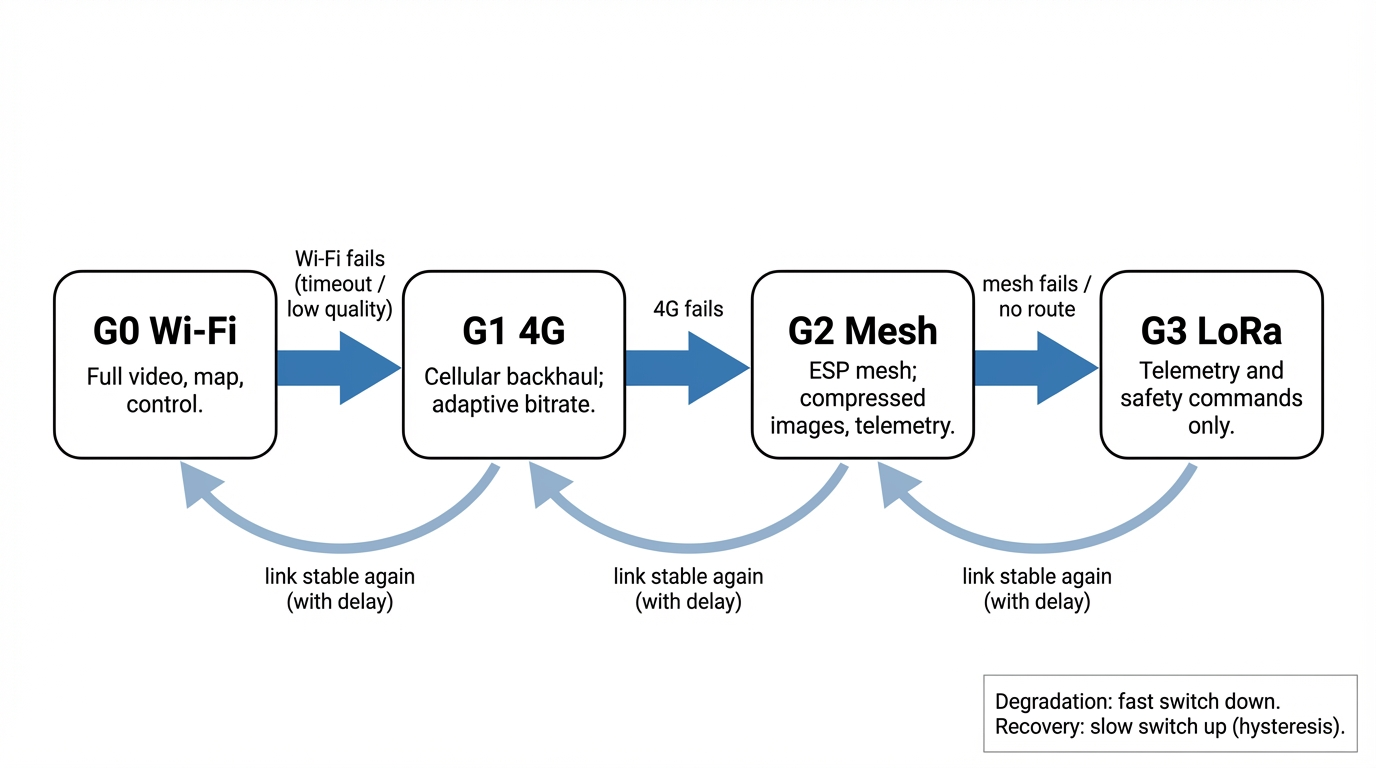
\includegraphics[width=0.95\textwidth,height=0.88\textheight,keepaspectratio]{figures/state_diagram.jpeg}
\vfill
\end{frame}

% --- Methodology Perception ---
\begin{frame}{Methodology: Perception}
\begin{itemize}
\item YOLOv8m: three parallel detectors --- fire/smoke (Kaggle dataset), extinguisher (Roboflow), person (COCO). Duplicate overlapping boxes from different heads are merged.
\item LLM (Llama-4-Scout via Groq): scene description, hazard severity, person re-ID
\item X-SDM: spatial decision memory (revisit vs new location); person profiling for map annotations
\item Heavy inference runs on the ground station; video streamed from UGV
\end{itemize}
\end{frame}

% --- Implementation platform ---
\begin{frame}{Implementation: Platform}
\begin{itemize}
\item Compute: Raspberry Pi~4 (8\,GB), Ubuntu 22.04, ROS~2 Humble
\item Sensors: YDLidar X3 (2D LiDAR, 10\,Hz), MPU6050 IMU, Kinect v1 (RGB-D for costmap), USB webcam + ESP32-CAM (720p, 15\,fps)
\item Comms: TP-Link Archer C6 (Wi-Fi AP), ESP32 DevKit mesh nodes, LoRa SX1278
\item Power: 24\,V pack (dual 3s3p 18650); $\sim$2\,h at 0.2\,m/s
\end{itemize}
\end{frame}

% --- UGV front, side, rear ---
\begin{frame}{UGV Platform: Front, Side, Rear}
\begin{columns}[T]
\begin{column}{0.32\textwidth}
\begin{center}
\includegraphics[width=\textwidth]{figures/ugv_front.jpg}\\
\small Front
\end{center}
\end{column}
\begin{column}{0.32\textwidth}
\begin{center}
\includegraphics[width=\textwidth]{figures/ugv_side.jpg}\\
\small Side
\end{center}
\end{column}
\begin{column}{0.32\textwidth}
\begin{center}
\includegraphics[width=\textwidth]{figures/ugv_back.jpg}\\
\small Rear
\end{center}
\end{column}
\end{columns}
\end{frame}

% --- Implementation stack ---
\begin{frame}{Implementation: Software Stack}
\begin{itemize}
\item ROS~2 Humble: Cartographer, Nav2, custom frontier package, rosbridge
\item Map preview for exploration: a small neural network (U-Net, ProxMaP family) looks at a local patch of the occupancy grid and guesses which unknown cells are probably free, so the robot prefers frontiers that look like doorways into open areas rather than blind alleys. It runs on a 128$\times$128 crop about once per second.
\item GCS: FastAPI backend, WebSocket (rosbridge), web dashboard (map, video, detections, teleop)
\end{itemize}
\end{frame}

% --- Test environment ---
\begin{frame}{Test Environment}
\begin{columns}
\begin{column}{0.5\textwidth}
\begin{itemize}
\item University department floor
\item $\sim$40\,m $\times$ 30\,m
\item Corridor, lobbies, rooms
\item Operator outside to simulate remote GCS
\end{itemize}
\end{column}
\begin{column}{0.5\textwidth}
\begin{center}
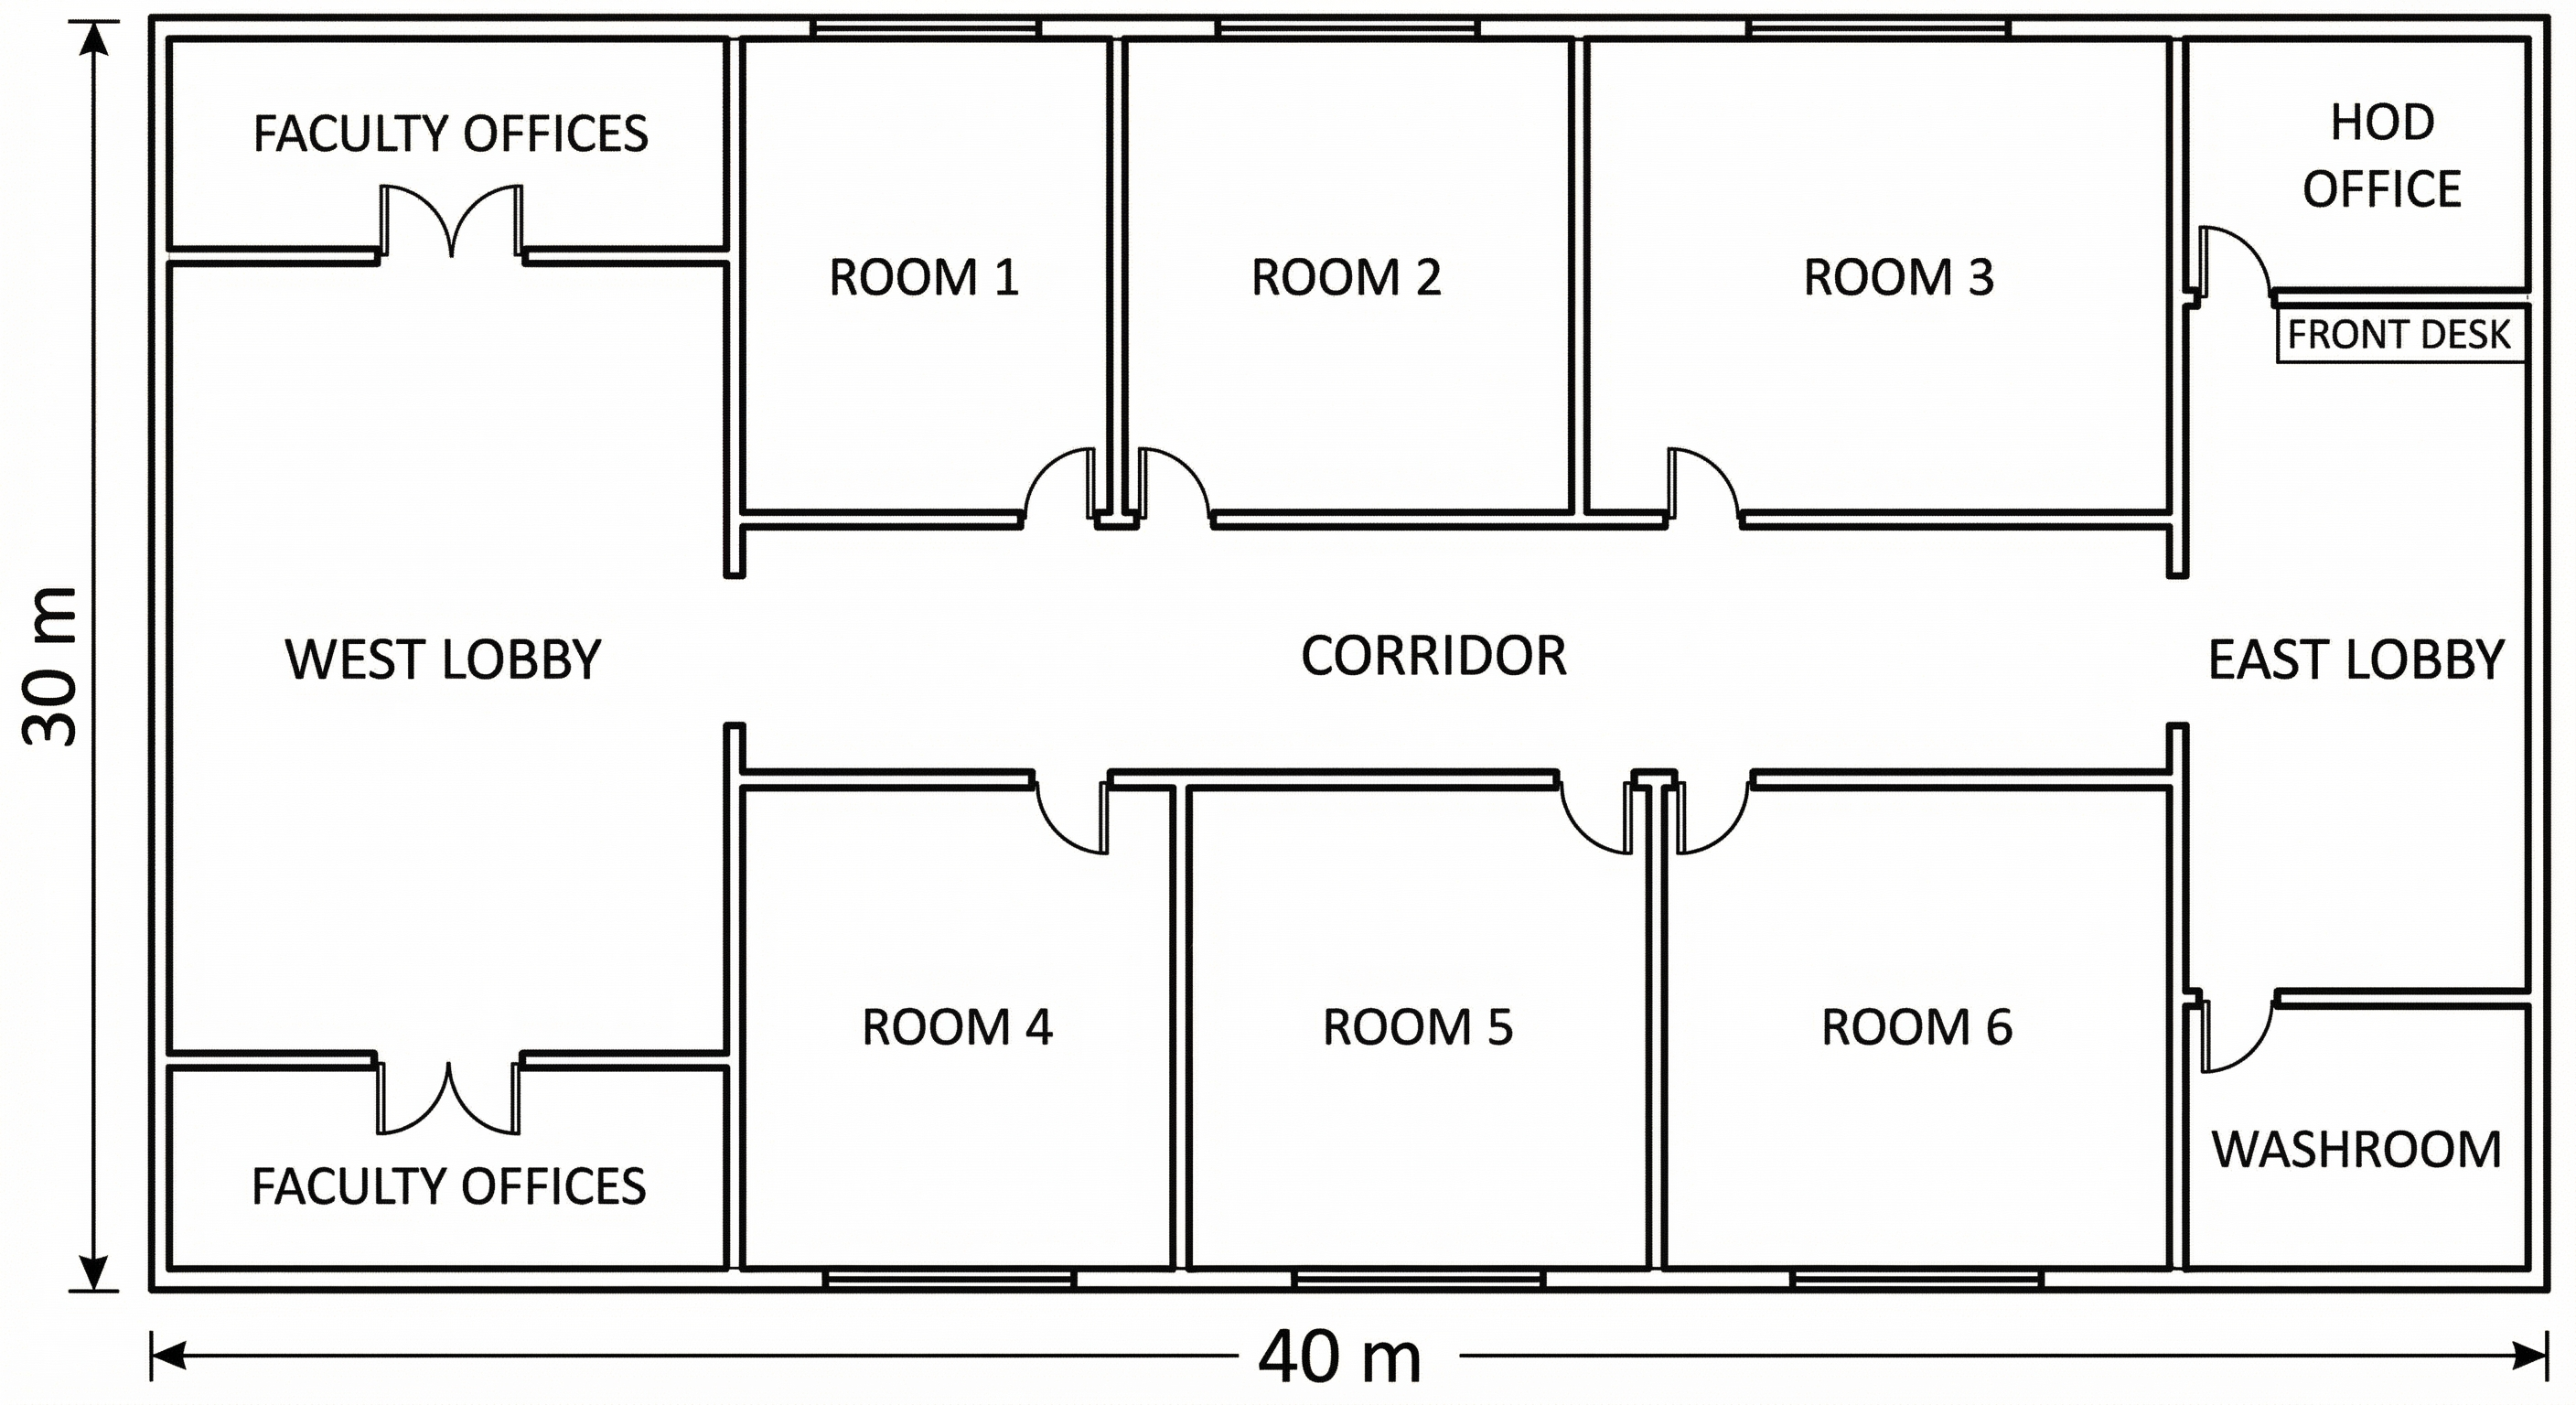
\includegraphics[width=\textwidth]{figures/floor_plan.jpeg}
\end{center}
\end{column}
\end{columns}
\end{frame}

% --- Results mapping ---
\begin{frame}{Early results: Mapping \& Exploration}
\begin{itemize}
\item SLAM: Cartographer runs on Pi~4 at 10\,Hz; map resolution 0.05\,m; qualitative drift lower where geometry is rich, higher in long corridors (quantitative ground-truth comparison planned)
\item Platform: $\sim$2\,h runtime at 0.2\,m/s in bench tests
\item Exploration: frontier + map preview integrated; pilot runs suggest faster coverage when the preview is on --- formal timed comparison deferred to final evaluation phase
\end{itemize}
\end{frame}

% --- Results communication ---
\begin{frame}{Early results: Communication}
\begin{itemize}
\item Wi-Fi and 4G: sufficient for video and map updates when LoS / in coverage (spot checks only so far)
\item Mesh fallback: usable for compressed snapshots and telemetry; throughput much lower than Wi-Fi --- fine-tuning ongoing
\item LoRa: basic indoor range checks for telemetry / return-to-base
\item Next: repeat measurements under a fixed test protocol for the final report
\end{itemize}
\end{frame}

% --- Results perception ---
\begin{frame}{Early results: Perception}
\begin{itemize}
\item Three YOLOv8m heads (fire/smoke, extinguisher, person) + Groq LLM + X-SDM: running on the ground station; dashboard shows map, video, detections
\item Latency feels interactive on Wi-Fi (order of hundreds of ms per stage) --- formal timing study still to do
\item Next: validation mAP on held-out data, failure cases, and mesh-path latency characterisation
\end{itemize}
\begin{center}
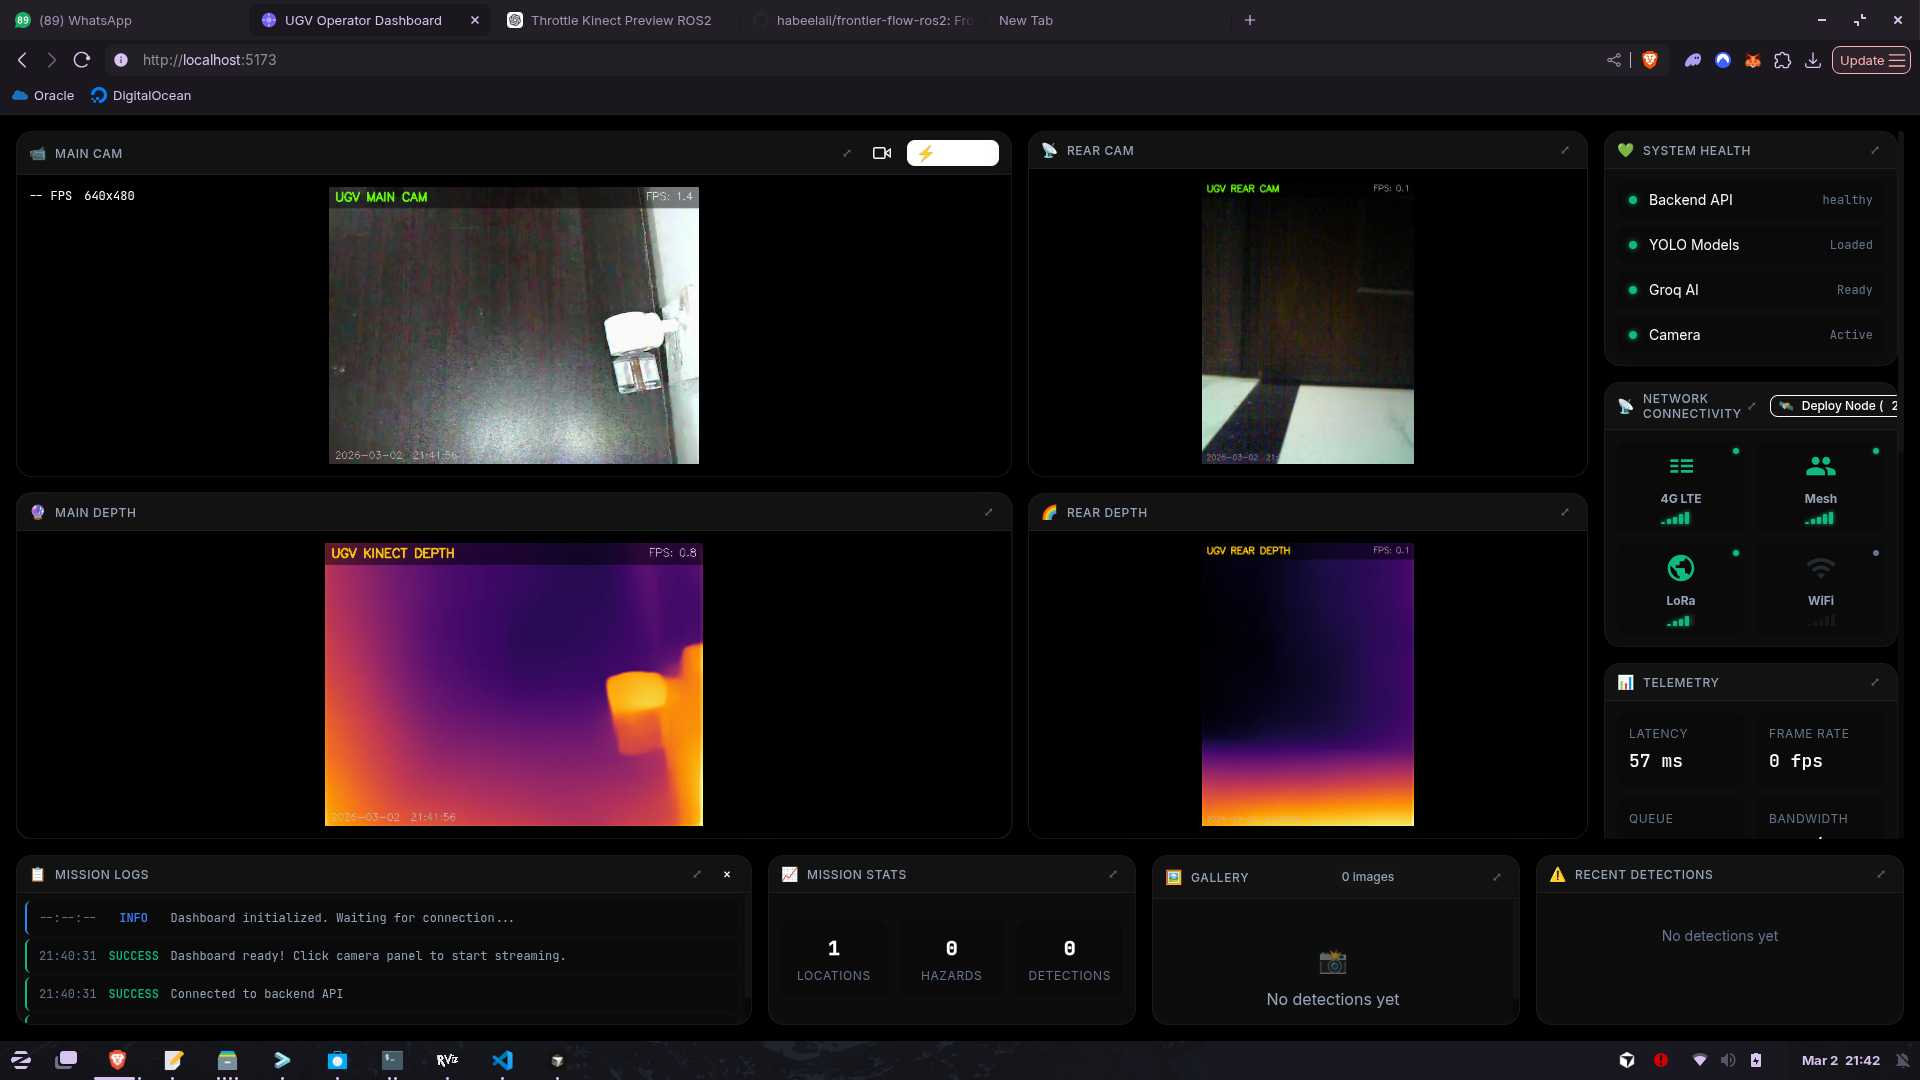
\includegraphics[width=0.5\textwidth]{figures/dashboard.png}
\end{center}
\end{frame}

% --- Remaining work ---
\begin{frame}{Remaining work (this semester)}
\begin{itemize}
\item Integration: close out minor tweaks on full stack (reliability, config, demo path)
\item Testing: structured KPI runs (mapping, comms tiers, perception) --- currently minimal / informal
\item Human factors: operator workload and usability (NASA-TLX, SUS, or similar)
\end{itemize}
\end{frame}

\begin{frame}{Longer-term extensions (optional)}
\begin{itemize}
\item 3D SLAM / multi-floor awareness
\item Multi-robot use of deployed mesh
\item Harsher environments (smoke, dust) and external evaluators
\end{itemize}
\end{frame}

% --- Conclusions (progress summary) ---
\begin{frame}{Progress summary}
\begin{itemize}
\item Architecture in place: Cartographer + Nav2 + frontier exploration with map preview (ProxMaP / U-Net) + multi-tier comms + GCS (YOLOv8m, LLM, X-SDM)
\item Hardware: RPi~4 (8\,GB), deployable mesh nodes; perception on the ground station for long runtime on the robot
\item Mid-semester: core demo works; final integration, fuller evaluation, and workload study still on the roadmap
\end{itemize}
\end{frame}

\begin{frame}{Thank you}
\begin{center}
\Huge Thank You
\end{center}
\end{frame}

\end{document}
